The vision layer controls all of the input from what our project sees. Our current design contains two cameras, one infrared / visible camera and one 3D camera. These two devices will be connected to the main computer (Raspberry Pi) via an interface. While this may not be the best configuration, it allows us to use the IR/Visible camera for detection and the 3D camera to determine the distance between the camera and the vehicle. This is currently the method that we think would work best for capturing the speed of the vehicle. We will also be considering any final methods for capturing the speed before purchasing the 3D camera and implementing it into the system. 

\subsection{Infrared / Visible Light Camera}
This subsystem is for finding each car in sight of the camera. Because it is an infrared and a visible light camera, it will be able to see the street even when cars are driving by. Inside the camera itself are two filters, one for visible light and one for infrared light. These two filters are controlled automatically by the camera and can automatically switch when it is no longer bright enough to see any vehicles. From this camera is a connection to the Vision interface so that if another part of the system needs access to the camera, it can get access through that interface.

\begin{figure}[h!]
	\centering
 	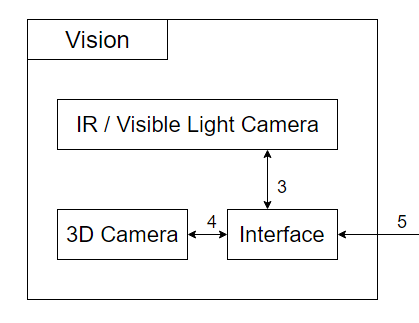
\includegraphics[width=0.60\textwidth]{images/vision_subsystem.png}
 \caption{IR / Visible light subsystem diagram}
\end{figure}

\subsubsection{Assumptions}
We are assuming that the cameras would be able to pick up the cars accurately enough to determine their location on screen. 

\subsubsection{Responsibilities}
The responsibility of the IR / Visible light camera is to be able to see what is in front of it regardless of the amount of light available.

\subsubsection{Subsystem Interfaces}

\begin {table}[H]
\caption {IR / Visible light subsystem interfaces} 
\begin{center}
    \begin{tabular}{ | p{1cm} | p{6cm} | p{3cm} | p{3cm} |}
    \hline
    ID & Description & Inputs & Outputs \\ \hline
    \#1 & Provide video feed from the IR / visible light camera to the interface & \pbox{3cm}{N/A} & \pbox{3cm}{Interface}  \\ \hline
    \end{tabular}
\end{center}
\end{table}

\subsection{3D Camera}
This subsystem is for finding the distance from the camera to any point on the screen. This will be helpful in providing the distance between two points on the frame so that we can more accurately find the distance the vehicle travels. From this camera is a connection to the Vision interface so that if another part of the system needs access to the camera, it can get access through that interface.

\begin{figure}[h!]
	\centering
 	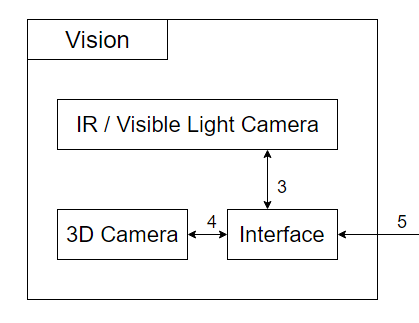
\includegraphics[width=0.60\textwidth]{images/vision_subsystem.png}
 \caption{3D camera subsystem diagram}
\end{figure}

\subsubsection{Assumptions}
We are assuming that the cameras would be able to pick up the cars accurately enough to determine their distance to the camera. 

\subsubsection{Responsibilities}
The responsibility of the 3D camera is to be able to calculate the distance from a point on the frame to the camera. We are also assuming that the camera will be able calculate the distance to the camera and thus the distance between two points on the screen.

\subsubsection{Subsystem Interfaces}

\begin {table}[H]
\caption {3D camera subsystem interfaces} 
\begin{center}
    \begin{tabular}{ | p{1cm} | p{6cm} | p{3cm} | p{3cm} |}
    \hline
    ID & Description & Inputs & Outputs \\ \hline
    \#2 & Provide video feed from the 3D camera to the interface & \pbox{3cm}{N/A} & \pbox{3cm}{Interface}  \\ \hline
    \end{tabular}
\end{center}
\end{table}

\subsection{Vision Interface}
This subsystem is for communicating camera frames outside of the vision system.

\begin{figure}[h!]
	\centering
 	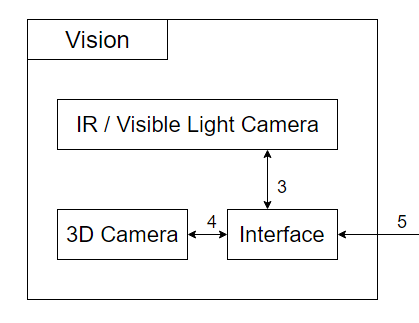
\includegraphics[width=0.60\textwidth]{images/vision_subsystem.png}
 \caption{Vision interface subsystem diagram}
\end{figure}

\subsubsection{Assumptions}
N/A

\subsubsection{Responsibilities}
Transfer information from the cameras to any other system that needs to use it.

\subsubsection{Subsystem Interfaces}

\begin {table}[H]
\caption {Vision interface subsystem interfaces} 
\begin{center}
    \begin{tabular}{ | p{1cm} | p{6cm} | p{3cm} | p{3cm} |}
    \hline
    ID & Description & Inputs & Outputs \\ \hline
    \#3 & Transfer Camera information outside of the vision system & \pbox{3cm}{3D camera, IR/visible light camera, Computer Interface} & \pbox{3cm}{Computer Interface}  \\ \hline
    \end{tabular}
\end{center}
\end{table}
